% 25/11/2008
% Alain Matthes
\documentclass{minimal}

\usepackage{tikz}
\usetikzlibrary{through,calc}
\usepackage{verbatim}

\begin{comment}

:Title: Lune of Hippocrates
:Author: Alain Matthes

What is the relationship between the area of the `isosceles right triangle`_ ABC and the
`area of the lune`_?

.. _isosceles right triangle: http://mathworld.wolfram.com/IsoscelesRightTriangle.html
.. _area of the lune: http://mathworld.wolfram.com/Lune.html
\end{comment}


\begin{document}

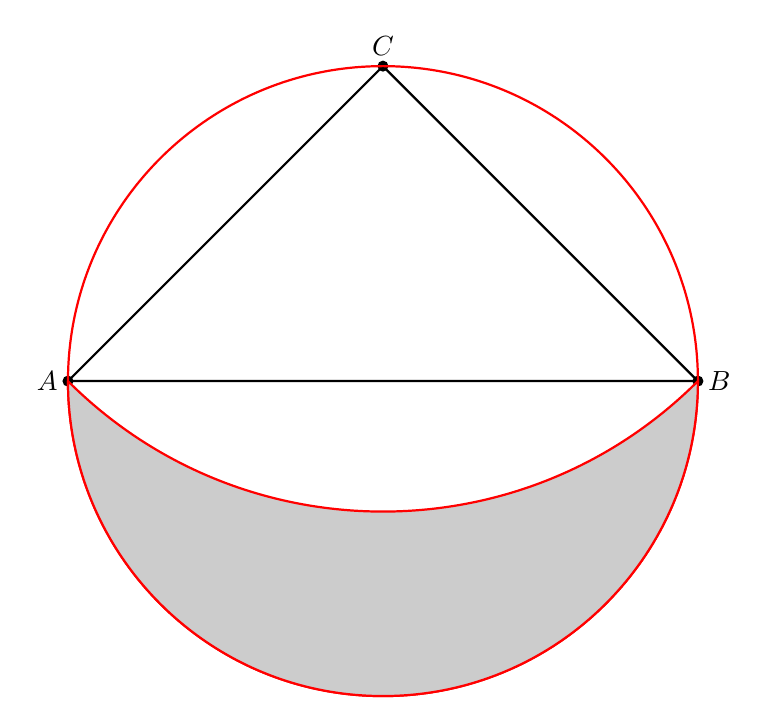
\begin{tikzpicture}[thick]
    \path[draw] (-4,0)  coordinate [label= left:$A$] (A)
            -- ( 0,4)  coordinate [label=above:$C$] (C)
            -- ( 4,0)  coordinate [label=right:$B$] (B)
            -- cycle;
    \foreach \point in {A,B,C}
           \fill [black] (\point) circle (2pt);
    \draw [color=red] circle(4cm);
    % The radius of the inner circular arc is equal to the length of BC.
    % Use the math engine to do the necessary calculations and store the
    % radius in the \n1 register
    \draw[color=red,fill=black!20]
         let \p1 = ($ (B) - (C) $),
             \n1 = {veclen(\x1,\y1)} in
         (A) arc (180:360:4cm) arc (-45:-135:\n1);
\end{tikzpicture}
\end{document}